\section{Алгоритм нахождения самопересечений} \label{ch3:selfCollision}
	Как было сказано ранее в параграфе \ref{ch2:pbd-improvments}, авторами оригинальной статьи уже был предложен алгоритм обнаружения самоперечений, однако построение сложной структуры, представленной в \cite{teschner2003optimized}, является слишком долгой операцией для выполнения на GPU, особенно для систем симуляции реального времени. В связи с этим, был разработан и реализован другой алгоритм обнаружения самопересечений.
	
	Во-первых, вместо обработки пересечений частиц и треугольников, было принято решение реализовать обработку пересечений двух частиц на основании того, что каждая частица задана сферой. При этом, радиусы упомянутых сфер выбираются таким образом, чтобы они были не меньше, чем половина длины покоя струтурного ограничения. Помимо этого, самопересечения между частицами, непосредственно соединенными структурными ограничениями или ограничениями сдвига - не проверяются, так как их положение уже задается при помощи ограничений.
	
	Во-вторых, для обнаружения соседних частиц используется алгоритм пространственного хеширования\cite{hashing2023}, в котором трехмерное пространство разбивается на ячейки, и номера этих ячеек пространства выступают в качестве ключа. Идея данного алгоритма заключается в создании двух массивов: первый ($Pointers$) будет хранить индексы частиц в глобальном списке частиц, а второй ($HashMap$) будет для каждой ячейки пространства хранить индекс в массиве $Pointers$, соответствующий первому из элементов, лежащих в данной ячейке пространства. Таким образом, для того, чтобы перебрать все элементы, принадлежащие данной ячейке пространства, достаточно получить индекс ячейки пространства в массиве $HashMap$ (назовем этот индекс $hash$), а затем рассмотреть все элементы массива $Pointers$ начиная с элемента под номером $HashMap[hash]$ (включительно) и до элемента $HashMap[hash + 1]$ (не включительно). Преимуществом данного алгоритма хеширования является то, что для построения данной хеш-таблицы не требуется сортировок, или других задач, параллельное решение которых невозможно или не имеет смысла, вместо них в данном алгоритме применяется лишь префиксная сумма, для которой уже разработаны алгоритмы параллельного вычисления (например представленный в \cite{hillis1986data}). Недостатком данной хеш-таблицы является то, что при её использовании отсутствует возможность динамического добавления и удаления, однако в рамках поставленной задачи это не требуется.
	
	В третьих, вместо того, чтобы записывать в хеш-таблицу только частицы, расположенные в соответствующей ячейке пространства, было принято решение дополнительно записывать ещё и частицы, расположенные в соседних ячейках. Данное изменение не влияет на объем памяти, занимаемый хеш-таблицей, но позволяет существенно уменьшить количество обращений к глобальной памяти на этапе обработки соседних вершин.
	
		
	\begin{figure}[ht!] 
		\center
		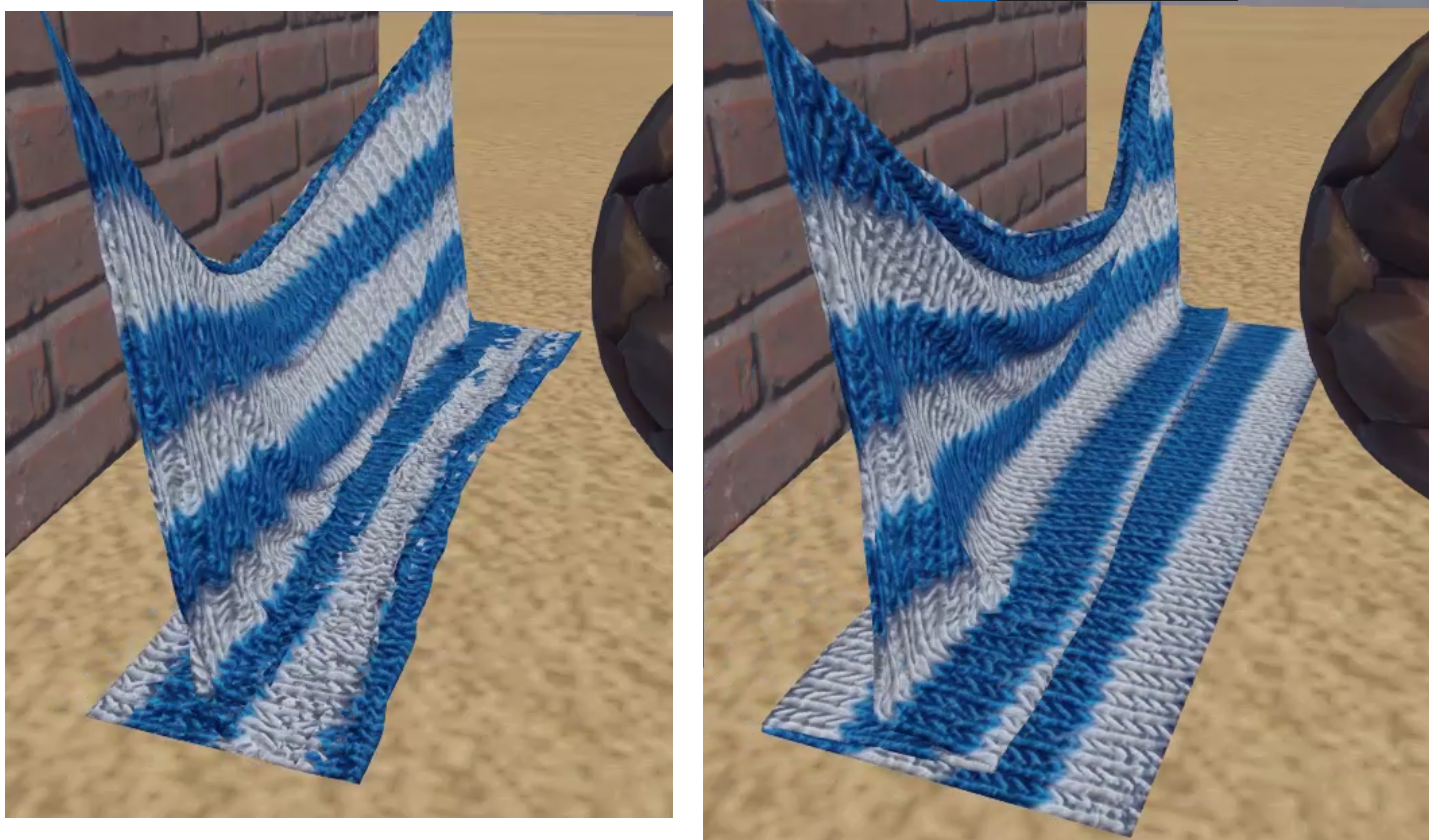
\includegraphics [scale=0.45] {my_folder/images//selfCollisionOffOn}
		\caption{Сравнение поведения симулируемой ткани с применением алгоритма самопересечения и без него. На рисунке слева проверка самопересечений не производится, а на рисунке справа используется описанный алгоритм.}
		\label{fig:selfCollision}  
	\end{figure}	
	\FloatBarrier

%% Вспомогательные команды - Additional commands
%
%\newpage % принудительное начало с новой страницы, использовать только в конце раздела
%\clearpage % осуществляется пакетом <<placeins>> в пределах секций
%\newpage\leavevmode\thispagestyle{empty}\newpage % 100 % начало новой страницы